\section{Existing vertical jump calculators}
There are few \textit{modern} jump calculators on the market right now. None are combined with existing fitness platforms -
our research shows all of them being standalone mobile or web applications (\labelcref{research:fitness-meter,research:whats-my-vert,research:my-jump}).
\par
There are multiple methods of measuring jump height, often this is important to athletes 
where success is caused/correlated with jump ability i.e. Sprinting \cite{jump-sprint-link}, American football, Basketball, Volleyball.
We also know vertical jump is an important test to assess the explosive strength of the leg
musculature of athletes \cite{aspects-of-strength,nsa-strength-in-athletes}.
We'll be using the time-in-air (TIA) to estimate jump height. Whilst this is inevitably not perfectly
accurate, when using a force plate \footnote{A measuring instrument that measures the ground reaction forces generated by somebody.}
it is no worse than other methods (in terms of consistency) \cite{measuring-jump-paper}.
Thereby still proving useful to the target demographic.
\par
To summarise, the vertical jump calculator created for the project is intended for use as a measurement of progress
and not a concrete result. There will be some deviation from other measurements (such as using a \href{https://www.topendsports.com/testing/products/vertical-jump/vertec.htm}{Vertec}).
\pagebreak 

\subsection{Maths behind calculating vertical jump using video}
\label{research:jump-maths}
Below we'll be considering the mathematics involved in finding vertical jump height using
\textbf{only smartphone video footage}.
\par
To explain the forces demonstrated in a countermovement jump (CMJ)\footnote{A vertical jump test performed by having an athlete quickly squat to a self-selected depth and then jump as high as possible.}
we'll be considering the 5 phases of action involved (\cref{fig:jump-phases}).
\begin{figure}[H]
	\centering
	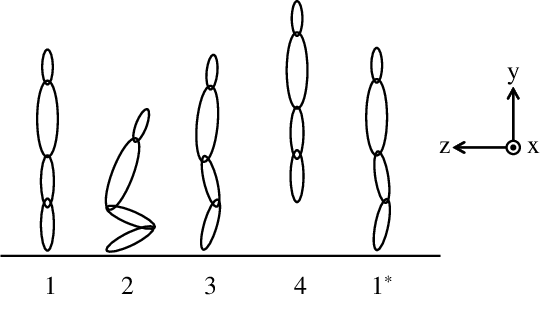
\includegraphics[width=0.5\linewidth]{jump-maths/phases-of-cmj.png}
	\caption{The sequence of actions involved in a CMJ.}
	\label{fig:jump-phases}
\end{figure}
\vspace*{-5mm}
\begin{figure}[H]
	\centering
	\resizebox{0.7\linewidth}{!}{
    \noindent
    \begin{tikzpicture}[trim left=0cm]
        \centering
        \begin{axis}[
                axis on top,
                axis lines = left,
                xlabel = {time in seconds (s)},
                ylabel = {Force in Newtons},
                xmin=-1, xmax=1,
                ymin=0, ymax=2600,
                xtick={-1.0,-0.5,0.0,0.5,1.0},
                ytick={500,1000,1500,2000},
                axis line style={opaque},
                label style={font=\tiny},
                ticklabel style={font=\tiny},
                tick style={draw=none},
                legend style={draw=none},
            ]

            % Define axis lines
            % Gravity line defined
            \path [
                name path=axis,
            ]
            (axis cs:-1,0) -- (axis cs:1,0);


            % Gravity line defined
            \addplot [
                name path=gravity,
                color=gray,
                fill=gray!10!,
                draw=none,
                area legend,
            ]
            {1000};

            %Below the main force of jumper is defined
            \addplot [
                name path=A,
                domain=-1:1,
                samples=11,
                color=red,
                smooth,
                line width=1pt,
                tension={0.15}
            ]
            coordinates {
                    (-1,1000)(-0.6,1000)(-0.5,500)(-0.4,1000)(-0.3,1500)(-0.2,2000)(0.0,0.0)(0.5,0.0)(0.6,2100)(0.7,1250)(0.8,1600)(0.9,1000)(1,1000)
                };

            \addplot [
                name path=phase2end,
                domain=-0.6:-0.4,
                samples=11,
                opacity=0,
            ]
            coordinates {
                    (-0.4,1000)(-0.35,1250)(-0.205,2000)(0.0,0.0)(0.5,0.0)(0.6,2100)(0.7,1250)(0.8,1600)(0.9,1000)(1,1000)
                };

            \addplot [
                name path=phase3start,
                domain=-0.4:-0.2,
                samples=11,
                opacity=0,
            ]
            coordinates {
                    (-0.25,1000)(-0.25,1750)(-0.205,2000)(0.0,0.0)(0.5,0.0)(0.6,2100)(0.7,1250)(0.8,1600)(0.9,1000)(1,1000)
                };

            \addplot [
                name path=phase4start,
                domain=-0.4:-0.2,
                samples=11,
                opacity=0,
            ]
            coordinates {
                    (-0.1,1000)(0.0,0.0)(0.5,0.0)(0.6,2100)(0.7,1250)(0.8,1600)(0.9,1000)(1,1000)
                };


            \addplot [
                domain=0:0.5,
                samples=11,
                color=red,
                line width=2pt,
            ]
            coordinates {
                    (0,0)(0.5,0)
                };

            % Coloring the phase 1 decline blue
            \addplot [
                fill=blue,
                fill opacity = 0.2,
            ]
            fill between[
                    of=A and phase2end
                ];
            % Coloring the phase 1 incline orange
            \addplot [
                fill=orange,
                fill opacity = 0.2,
            ]
            fill between[
                    of=phase2end and phase3start
                ];
            % Coloring the phase 3 decline orange
            \addplot [
                fill=yellow,
                fill opacity = 0.2,
            ]
            fill between[
                    of=phase3start and phase4start
                ];
            % Coloring final phase
            \addplot [fill=green,fill opacity = 0.2] fill between[
                    of=A and gravity, soft clip={domain=0.55:1}
                ];

            % Coloring the gravity line
            \addplot [gray!10!] fill between[
                    of=A and axis, soft clip={domain=-1:-0.4}
                ];
            \addplot [gray!10!] fill between[
                    of=gravity and axis, soft clip={domain=-0.4:-0.1}
                ];
            \addplot [gray!10!] fill between[
                    of=A and axis, soft clip={domain=-0.1:0.55}
                ];
            \addplot [gray!10!] fill between[
                    of=gravity and axis, soft clip={domain=0.55:1}
                ];

            \legend{
                \tiny Force of Gravity,
                \tiny Force of Jumper Movement,
            }


            % The phase 1 bending label (70Ns)
            \addplot[mark=none, color = blue] coordinates {(-0.475,930)} node[pin=100:{\tiny 70Ns}]{} ;
            % Phase grey marks
            \addplot[mark=*, color=black!80!, draw opacity = 0] coordinates {(-0.6,1000)(-0.4,1000)(-0.26,1750)(0,0)(0.5,0)};
            % The phase 2 label (70Ns)
            \addplot[mark=none, color = orange] coordinates {(-0.31,1250)} node[pin=100:{\tiny 70Ns}]{} ;
            % The phase 3 label (245Ns)
            \addplot[mark=none, color = yellow] coordinates {(-0.16,1250)} node[pin=80:{\tiny 245Ns}]{} ;
            % The phase 4 label (245Ns)
            \addplot[mark=none, color = green] coordinates {(0.600,1250)} node[pin=100:{\tiny 245Ns}]{} ;


        \end{axis}
    \end{tikzpicture}}
	\caption{Ground reaction forces during vertical jump.}
	\label{fig:jump-phases-graph}
\end{figure}
\par
We'll use a simplified example of a force plate analysis (\todo[color=purple]{reference graph}). In reality the force curve won't be so smooth
but this should demonstrate the phases quite clearly. 



\[\displaystyle F = m * g\]
\[
	\displaystyle
	\begin{aligned}
	981 N &= m * 9.81 m/s^2 \\ \\
	=> m &= \frac{981N}{9.81 m/s^2} = 100kg
	\end{aligned}	
\]

$$F_{Jumper} = F_{GRF} - F_{Gravity} <=0$$

\[F = m a => F t = m a t
\]
Because F is not constant but a function of time, and $v =a t$:
\par
$$\displaystyle
=> \int_{t_1}^{t_2} F_{Jumper}(t) \mathrm{d}t = m v$$

\[\displaystyle
\begin{aligned}
\int_{t_1}^{t_2} F(t) \mathrm{d}t = m v\\ \\
=> -70 N s = 100kg * v\\
=> v = -70 N s / 100kg = -0.7 m/s
\end{aligned}
\]


\subsection{FitnessMeter - Test \& Measure}
\label{research:fitness-meter}
\subsection{What's My Vertical?}
\label{research:whats-my-vert}
\subsection{My Jump 2}
\label{research:my-jump}


\begin{itemize}
	\item \href{https://www.thehoopsgeek.com/measurement-app/#manual}{HoopsGeek App}
	\item \href{https://apps.apple.com/us/app/fitnessmeter-test-measure/id477488986}{Old ass iphone app}
	\item \href{https://apps.apple.com/gb/app/my-jump-2/id1148617550#?platform=iphone}{MyJump2 itunes}
	\item \href{https://www.youtube.com/watch?v=tIBiHDyev6w}{MyJump2 in use}
	\item \href{https://www.topendsports.com/testing/products/vertical-jump/video.htm}{Maths}
	\item \href{https://www.thehoopsgeek.com/the-physics-of-the-vertical-jump/}{Detailed maths courtesy of thehoopsgeek - legend}
\end{itemize}